\documentclass{report}
\usepackage{graphicx, tikz-cd, float, titlepic, booktabs} % Required for inserting images
\usepackage{pgfplots}
\usepackage{multicol}
\usepackage{makecell}
\pgfplotsset{compat=1.15}
\usepackage{mathrsfs}
\usetikzlibrary{arrows}
\usepackage{amsmath, amssymb, amsthm, amsfonts, siunitx, physics, gensymb}
\AtBeginDocument{\RenewCommandCopy\qty\SI}
\usepackage[version=4]{mhchem}
\usepackage[most,many,breakable]{tcolorbox}
\usepackage{xcolor, fancyhdr, varwidth}
\usepackage[Glenn]{fncychap}
%Options: Sonny, Lenny, Glenn, Conny, Rejne, Bjarne, Bjornstrup
\usepackage{hyperref, cleveref}
\usepackage{icomma, enumitem} %comma as decimal and continue enumerate with [resume]
\usepackage{plimsoll} %use standard state symbol with \stst
\usepackage[danish]{babel}
\renewcommand{\cellalign}{cl}
\renewcommand{\theadalign}{cl}
\renewcommand\theadfont{\bfseries}
%%%%%%%%%%%%%%%%%%%%%%%%%%%%%%
% SELF MADE COLORS
%%%%%%%%%%%%%%%%%%%%%%%%%%%%%%
\definecolor{myg}{RGB}{56, 140, 70}
\definecolor{myb}{RGB}{45, 111, 177}
\definecolor{myr}{RGB}{199, 68, 64}
\definecolor{mytheorembg}{HTML}{F2F2F9}
\definecolor{mytheoremfr}{HTML}{00007B}
\definecolor{mylenmabg}{HTML}{FFFAF8}
\definecolor{mylenmafr}{HTML}{983b0f}
\definecolor{mypropbg}{HTML}{f2fbfc}
\definecolor{mypropfr}{HTML}{191971}
\definecolor{myexamplebg}{HTML}{F2FBF8}
\definecolor{myexamplefr}{HTML}{88D6D1}
\definecolor{myexampleti}{HTML}{2A7F7F}
\definecolor{mydefinitbg}{HTML}{E5E5FF}
\definecolor{mydefinitfr}{HTML}{3F3FA3}
\definecolor{notesgreen}{RGB}{0,162,0}
\definecolor{myp}{RGB}{197, 92, 212}
\definecolor{mygr}{HTML}{2C3338}
\definecolor{myred}{RGB}{127,0,0}
\definecolor{myyellow}{RGB}{169,121,69}
\definecolor{myexercisebg}{HTML}{F2FBF8}
\definecolor{myexercisefg}{HTML}{88D6D1}
%%%%%%%%%%%%%%%%%%%%%%%%%%%%%%%%%%%%%%%%%%%%%%%%%%%%%%%%%%%%%%%%%%%%%%
% Box environments for theorems and problems
%%%%%%%%%%%%%%%%%%%%%%%%%%%%%%%%%%%%%%%%%%%%%%%%%%%%%%%%%%%%%%%%%%%%%
\setlength{\parindent}{1cm}
%================================
% Question BOX
%================================
\makeatletter
\newtcbtheorem{question}{Opgave}{enhanced,
	breakable,
	colback=white,
	colframe=myb!80!black,
	attach boxed title to top left={yshift*=-\tcboxedtitleheight},
	fonttitle=\bfseries,
	title={#2},
	boxed title size=title,
	boxed title style={%
			sharp corners,
			rounded corners=northwest,
			colback=tcbcolframe,
			boxrule=0pt,
		},
	underlay boxed title={%
			\path[fill=tcbcolframe] (title.south west)--(title.south east)
			to[out=0, in=180] ([xshift=5mm]title.east)--
			(title.center-|frame.east)
			[rounded corners=\kvtcb@arc] |-
			(frame.north) -| cycle;
		},
	#1
}{def}
\makeatother
%================================
% DEFINITION BOX
%================================

\newtcbtheorem[]{Definition}{Definition}{enhanced,
	before skip=2mm,after skip=2mm, colback=red!5,colframe=red!80!black,boxrule=0.5mm,
	attach boxed title to top left={xshift=1cm,yshift*=1mm-\tcboxedtitleheight}, varwidth boxed title*=-3cm,
	boxed title style={frame code={
					\path[fill=tcbcolback]
					([yshift=-1mm,xshift=-1mm]frame.north west)
					arc[start angle=0,end angle=180,radius=1mm]
					([yshift=-1mm,xshift=1mm]frame.north east)
					arc[start angle=180,end angle=0,radius=1mm];
					\path[left color=tcbcolback!60!black,right color=tcbcolback!60!black,
						middle color=tcbcolback!80!black]
					([xshift=-2mm]frame.north west) -- ([xshift=2mm]frame.north east)
					[rounded corners=1mm]-- ([xshift=1mm,yshift=-1mm]frame.north east)
					-- (frame.south east) -- (frame.south west)
					-- ([xshift=-1mm,yshift=-1mm]frame.north west)
					[sharp corners]-- cycle;
				},interior engine=empty,
		},
	fonttitle=\bfseries,
	title={#2},#1}{def}
\newtcbtheorem[]{definition}{Definition}{enhanced,
	before skip=2mm,after skip=2mm, colback=red!5,colframe=red!80!black,boxrule=0.5mm,
	attach boxed title to top left={xshift=1cm,yshift*=1mm-\tcboxedtitleheight}, varwidth boxed title*=-3cm,
	boxed title style={frame code={
					\path[fill=tcbcolback]
					([yshift=-1mm,xshift=-1mm]frame.north west)
					arc[start angle=0,end angle=180,radius=1mm]
					([yshift=-1mm,xshift=1mm]frame.north east)
					arc[start angle=180,end angle=0,radius=1mm];
					\path[left color=tcbcolback!60!black,right color=tcbcolback!60!black,
						middle color=tcbcolback!80!black]
					([xshift=-2mm]frame.north west) -- ([xshift=2mm]frame.north east)
					[rounded corners=1mm]-- ([xshift=1mm,yshift=-1mm]frame.north east)
					-- (frame.south east) -- (frame.south west)
					-- ([xshift=-1mm,yshift=-1mm]frame.north west)
					[sharp corners]-- cycle;
				},interior engine=empty,
		},
	fonttitle=\bfseries,
	title={#2},#1}{def}

\newtcbtheorem{theo}%
    {Theorem}{}{theorem}
\newtcolorbox{prob}[1]{colback=red!5!white,colframe=red!50!black,fonttitle=\bfseries,title={#1}}
%================================
% NOTE BOX
%================================

\usetikzlibrary{arrows,calc,shadows.blur}
\tcbuselibrary{skins}
\newtcolorbox{note}[1][]{%
	enhanced jigsaw,
	colback=gray!20!white,%
	colframe=gray!80!black,
	size=small,
	boxrule=1pt,
	title=\textbf{Note:},
	halign title=flush center,
	coltitle=black,
	breakable,
	drop shadow=black!50!white,
	attach boxed title to top left={xshift=1cm,yshift=-\tcboxedtitleheight/2,yshifttext=-\tcboxedtitleheight/2},
	minipage boxed title=1.5cm,
	boxed title style={%
			colback=white,
			size=fbox,
			boxrule=1pt,
			boxsep=2pt,
			underlay={%
					\coordinate (dotA) at ($(interior.west) + (-0.5pt,0)$);
					\coordinate (dotB) at ($(interior.east) + (0.5pt,0)$);
					\begin{scope}
						\clip (interior.north west) rectangle ([xshift=3ex]interior.east);
						\filldraw [white, blur shadow={shadow opacity=60, shadow yshift=-.75ex}, rounded corners=2pt] (interior.north west) rectangle (interior.south east);
					\end{scope}
					\begin{scope}[gray!80!black]
						\fill (dotA) circle (2pt);
						\fill (dotB) circle (2pt);
					\end{scope}
				},
		},
	#1,
}
%================================
% EXAMPLE BOX
%================================
\newtcbtheorem[number within=section]{Example}{Example}
{%
	colback = myexamplebg
	,breakable
	,colframe = myexamplefr
	,coltitle = myexampleti
	,boxrule = 1pt
	,sharp corners
	,detach title
	,before upper=\tcbtitle\par\smallskip
	,fonttitle = \bfseries
	,description font = \mdseries
	,separator sign none
	,description delimiters parenthesis
}
{ex}
%================================
% THEOREM BOX
%================================

\tcbuselibrary{theorems,skins,hooks}
\newtcbtheorem[number within=section]{Theorem}{Theorem}
{%
	enhanced,
	breakable,
	colback = mytheorembg,
	frame hidden,
	boxrule = 0sp,
	borderline west = {2pt}{0pt}{mytheoremfr},
	sharp corners,
	detach title,
	before upper = \tcbtitle\par\smallskip,
	coltitle = mytheoremfr,
	fonttitle = \bfseries\sffamily,
	description font = \mdseries,
	separator sign none,
	segmentation style={solid, mytheoremfr},
}
{th}

%%%%%%%%%%%%%%%%%%%%%%%%%%%%%%%%%%%%%%%%%%%%%%%%%%%%%%%%%%%%%%%%%
% SELF MADE COMMANDS
%%%%%%%%%%%%%%%%%%%%%%%%%%%%%%
\newcommand{\sol}{\setlength{\parindent}{0cm}\textbf{\textit{Løsning:}}\setlength{\parindent}{1cm}}
%%%%%%%%%%%%%%%%%%%%%%%%%%%%%%%%%
\usepackage[tmargin=2cm,rmargin=1in,lmargin=1in,margin=0.85in,bmargin=2cm,footskip=.2in]{geometry}\pagestyle{fancy}
\lhead{Minrui Kevin Zhou 3.b}
\rhead{Rapport 5 - Krystalviolet}

\title{Rapport 5 - Krystalviolet\\
{\Large \textbf{3.b kemi A}}}
\author{Kevin Zhou}
\date{\today}

\begin{document}
\titlepic{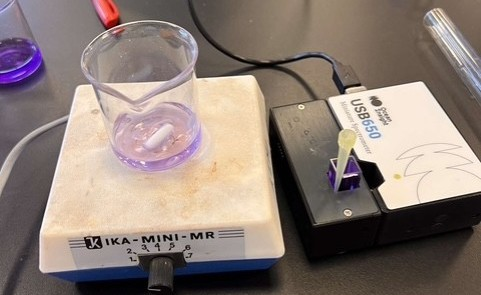
\includegraphics[width=0.7\textwidth]{close.jpg}}
\maketitle
\section*{Formål}
Formålet med eksperimentet er at bestemme hastighedsudtrykket for krystalviolets reaktion med hydroxid.
\section*{Teori}
Krystalviolet er en ionforbindelse, og strukturformlen ses i \cref{fig:krystalviolet}.
\begin{figure}[H]
\begin{center}
  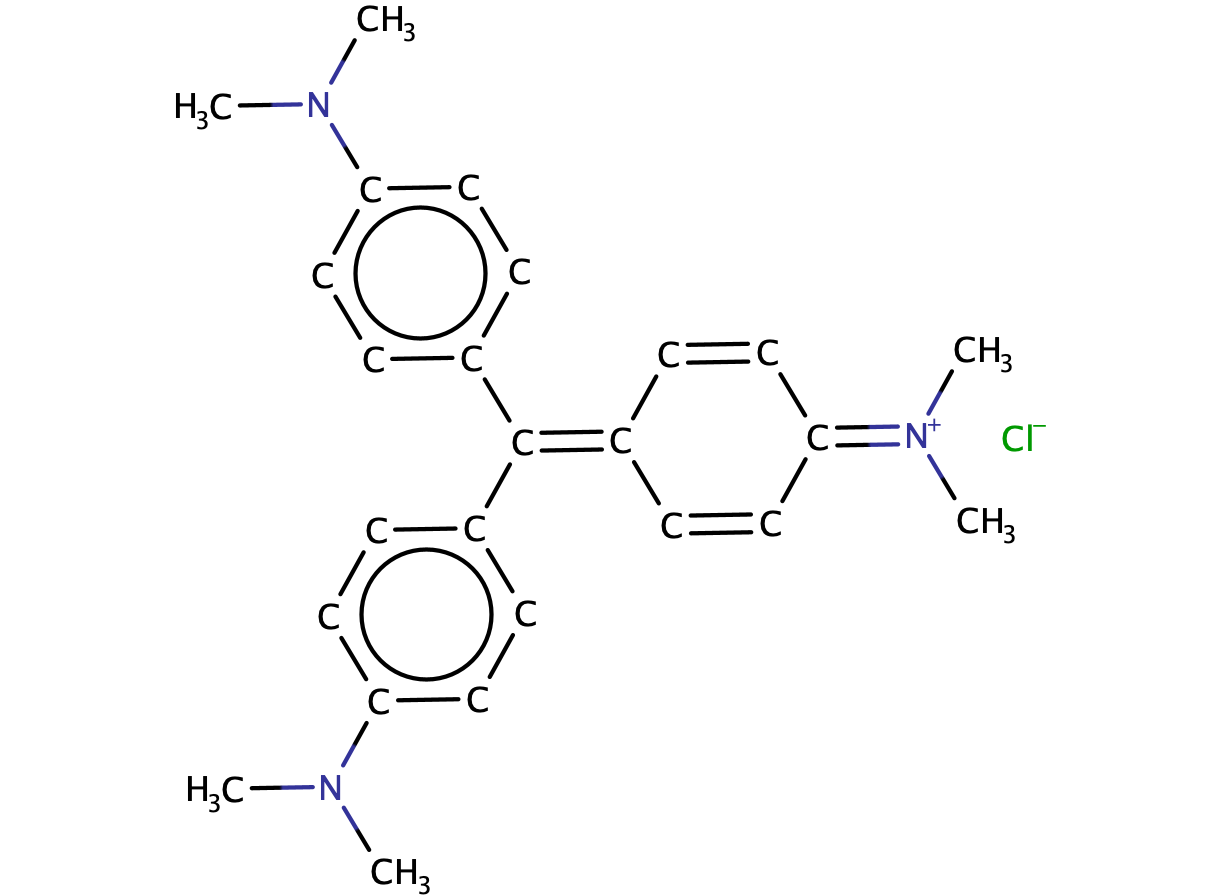
\includegraphics[width=0.5\textwidth]{krystalviolet.png}
\end{center}
\caption{Strukturen for krystalviolet tegnet i MarvinSketch}
\label{fig:krystalviolet}
\end{figure}
Det ses, at stoffet indeholder over 8 konjugerede dobbeltbindinger, og det må derfor være farvet.
Det passer med, at stoffet er violet.
Reaktionsskemaet for reaktionen mellem krystalviolet (eller formelt set dens positivet ion) og hydroxid ses i \cref{fig:reaktion}.
\begin{figure}[H]
\begin{center}
  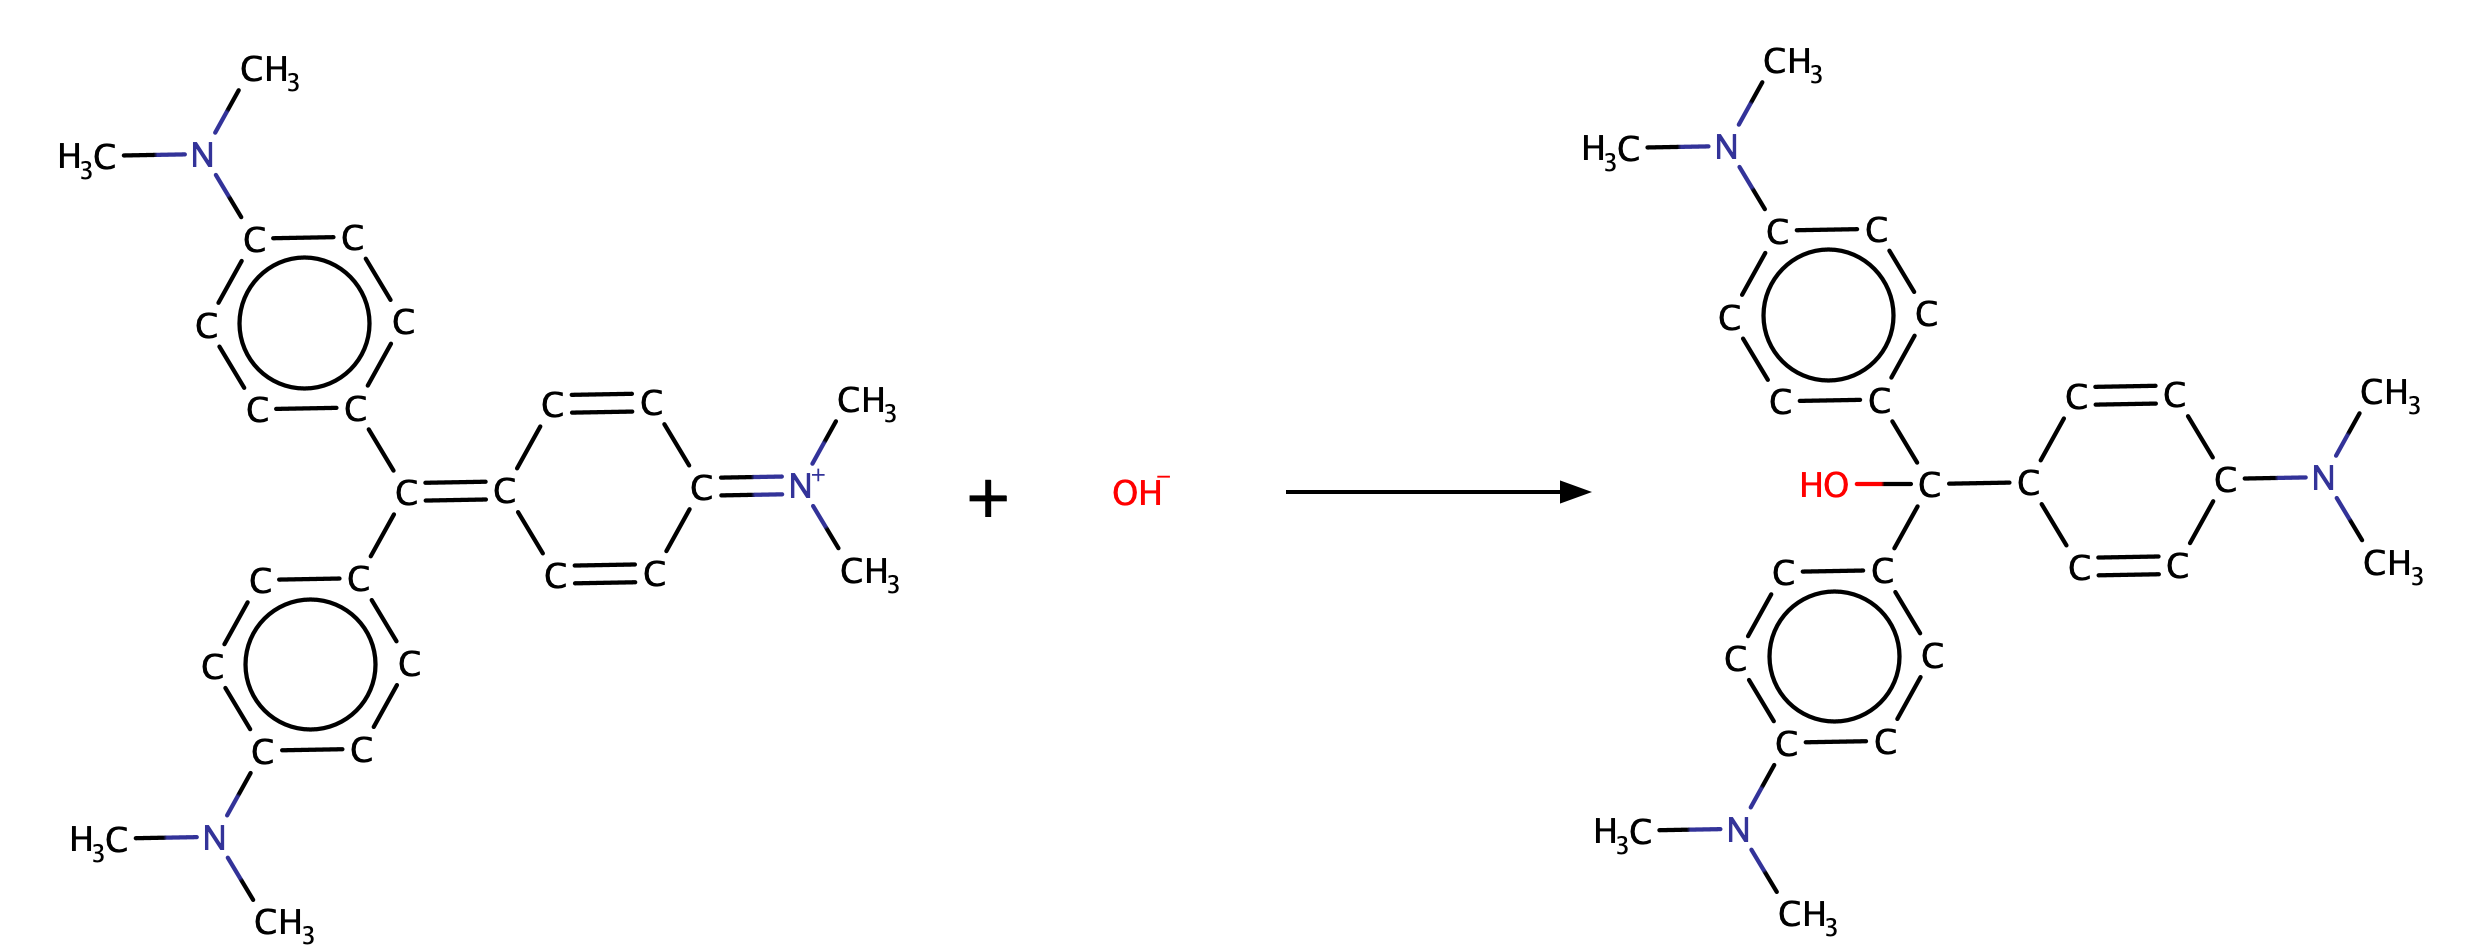
\includegraphics[width=\textwidth]{reaktion.png}
\end{center}
\caption{Reaktionbsskema for reaktion mellem krystalviolet og hydroxid}
\label{fig:reaktion}
\end{figure}
Ved reaktionen brydes blandt andet dobbeltbindingen midt i krystalviolets positive ion, så der ikke længere er mindst 8 konjugerede dobbeltbindinger, og produktet er derfor farveløst.
Derudover ser vi, at et generelt udtryk for reaktionshastigheden (som er den samme mht. krystalviolet og mht. hydroxid) må være
\[
v=k \cdot \left[\text{krystalviolet} \right] ^{x} \cdot \left[\ce{OH-} \right] ^{y}
\] 
hvor $v$ er reaktionshastigheden (bemærk at den er ens mht. krystalviolet og mht. hydroxid), $k$ er hastighedskonstanten, og $x,\;y \in \{z \in \mathbb{Z}: z \geq 0\}$.
Vi vil altså gerne bestemme $x$ og $y$. 

Siden vi fra Lambert-Beers lov har, at absorbansen er proportional med den aktuelle stofmængdekoncentration af det farvede stof i en opløsning;
\[
A=\varepsilon _{\lambda } \cdot l \cdot [\text{krystalviolet} ]
\] 
så kan vi nemt måle reaktionshastigheden via spektrofotometri.
Formindskelsen i absorbans pr. tid betegner vi $v^*$:
\begin{equation*}
\begin{split}
  v^* &=- \dv{A}{t}\\
  &=-c \cdot \dv{\left[\text{krystalviolet} \right]}{t}\\
  &=c \cdot v
\end{split}
\end{equation*}
hvor $c=\varepsilon _{\lambda } \cdot l$ er en konstant. 

Vi anvender i eksperimentet et stort overskud af hydroxid, så den aktuelle stofmængdekoncentration af hydroxid er nogenlunde konstant under reaktionen.
Produktet $k \cdot \left[\ce{OH-} \right] ^{y}$ er da konstant, og vi betegner det $k_1$.
Hastighedsudtrykket bliver så
\begin{equation*}
\begin{split}
  v &= k \cdot \left[\ce{OH-} \right] ^{y} \cdot \left[\text{krystalviolet} \right] ^{x}\\
  &=k_1 \cdot \left[\text{krystalviolet} \right] ^{x}
\end{split}
\end{equation*}
I del 2 halveres $\left[\ce{OH-} \right]$ ift. del 1, og vi kan da sammenligne de to $k_1$'er for at bestemme $y$.

\section*{Apparatur, kemikalier og sikkerhed}
\subsection*{Apparatur}
\begin{multicols}{3}
 \begin{itemize}
  \item Spektrofotometer
  \item Kuvetter
  \item Pipette, $10 \;\unit{mL} $ 
  \item Pipette, $2 \;\unit{mL} $
  \item 2 Pipetter, $1 \;\unit{mL} $
  \item Pipettesuger 
  \item Magnetomrører
  \item Magnet
  \item 2 bægerglas, $50 \;\unit{mL} $
  \item Plastpipetter 
  \item Reagensglas 
 \end{itemize} 
\end{multicols}
\subsection*{Kemikalier}
\begin{itemize}
  \item $2,00 \cdot 10 ^{-5} \;\unit{\textsc{m}} $ krystalviolet, \ce{C25H30ClN3} 
  \item $0,500 \;\unit{\textsc{m}} $ natriumhydroxid, \ce{NaOH} 
\end{itemize}
\subsection*{Sikkerhed}
\begin{itemize}
  \item $2,00 \cdot 10 ^{-5} \;\unit{\textsc{m}} $ krystalviolet er sundhedsskadeligt. 
  \item $0,500 \;\unit{\textsc{m}} $ natriumhydroxid virker ætsende.
\end{itemize}
\section*{Udførelse}
Til start tændes spektrofotometeret og kalibreres med demineraliseret vand.
Derefter fyldes en kuvette op med $2,00 \cdot 10 ^{-5} \;\unit{\textsc{m}} $ krystalviolet, og et absorptionsspektrum optages. 
Den bølgelængde, hvor absorbansen er maksimal noteres ned.
De efterfølgende absorbansmålinger måles ved denne bølgelængde.

\subsection*{Del 1}
$10,0 \;\unit{mL} $ $2,00 \cdot 10 ^{-5} \;\unit{\textsc{m}} $ krystalviolet afpippeteres til et $50 \;\unit{mL} $ bægerglas, hvori en magnet placeres og omrøres med magnetomrøreren. 
Herefter afpippeteres $2,00 \;\unit{mL} $ $0,500 \;\unit{\textsc{m}} $ natriumhydroxid til et reagensglas.
Reagensglassets indhold hældes herefter på én gang over i bægerglasset med opløsningen af krystalviolet.
Noget af reaktionsblandingen overføres så hurtigt til en kuvette, hvorefter den placeres i spektrofotometeret og en måling af reaktionsblandingens absorbans startes.
Opstillingen ses i \cref{fig:opstilling}.
\begin{figure}[H]
\begin{center}
  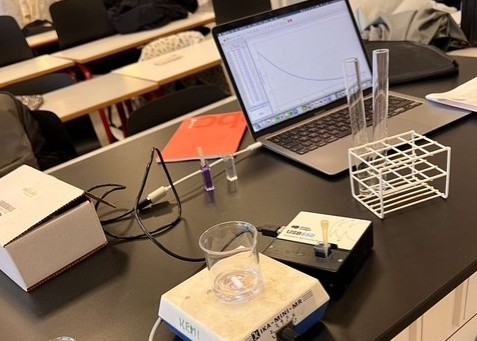
\includegraphics[width=\textwidth]{opstilling.jpg}
\end{center}
\caption{Reaktionsblandingen overføres hurtigt til en kuvette, der placeres i spektrofotometeret}
\label{fig:opstilling}
\end{figure}
\subsection*{Del 2}
Del 1 gentages, men hvor $1,00 \;\unit{mL} $ demineraliseret vand og $1,00 \;\unit{mL} $ $0,500 \;\unit{\textsc{m}} $ \ce{NaOH} afpippeteres til reagensglasset i stedet.
\section*{Resultater}
Ved det optagne absorptionsspektrum for krystalviolet-opløsningen bestemte vi bølgelængden, hvor absorbansen er maksimal, til at være $589 \;\unit{nm} $, hvilket fremgår af nedenstående tabel.
\begin{table}[H]
  \centering
  \begin{tabular}{@{}l@{}}
  \toprule
  \thead{Bølgelængde $\lambda $, hvor absor-\\bansen er maksimal/nm} \\
  \midrule
  589\\
  \bottomrule
  \end{tabular}
\end{table}
Måleresultaterne for del 1 og del 2 fylder så meget, at de her udelades, men vedhæftes seperat i lectio.
Dog ses $(t,A)$-graferne for del 1 og del 2 i hhv. \cref{fig:del1} og \cref{fig:del2}.
\begin{figure}[H]
\begin{center}
  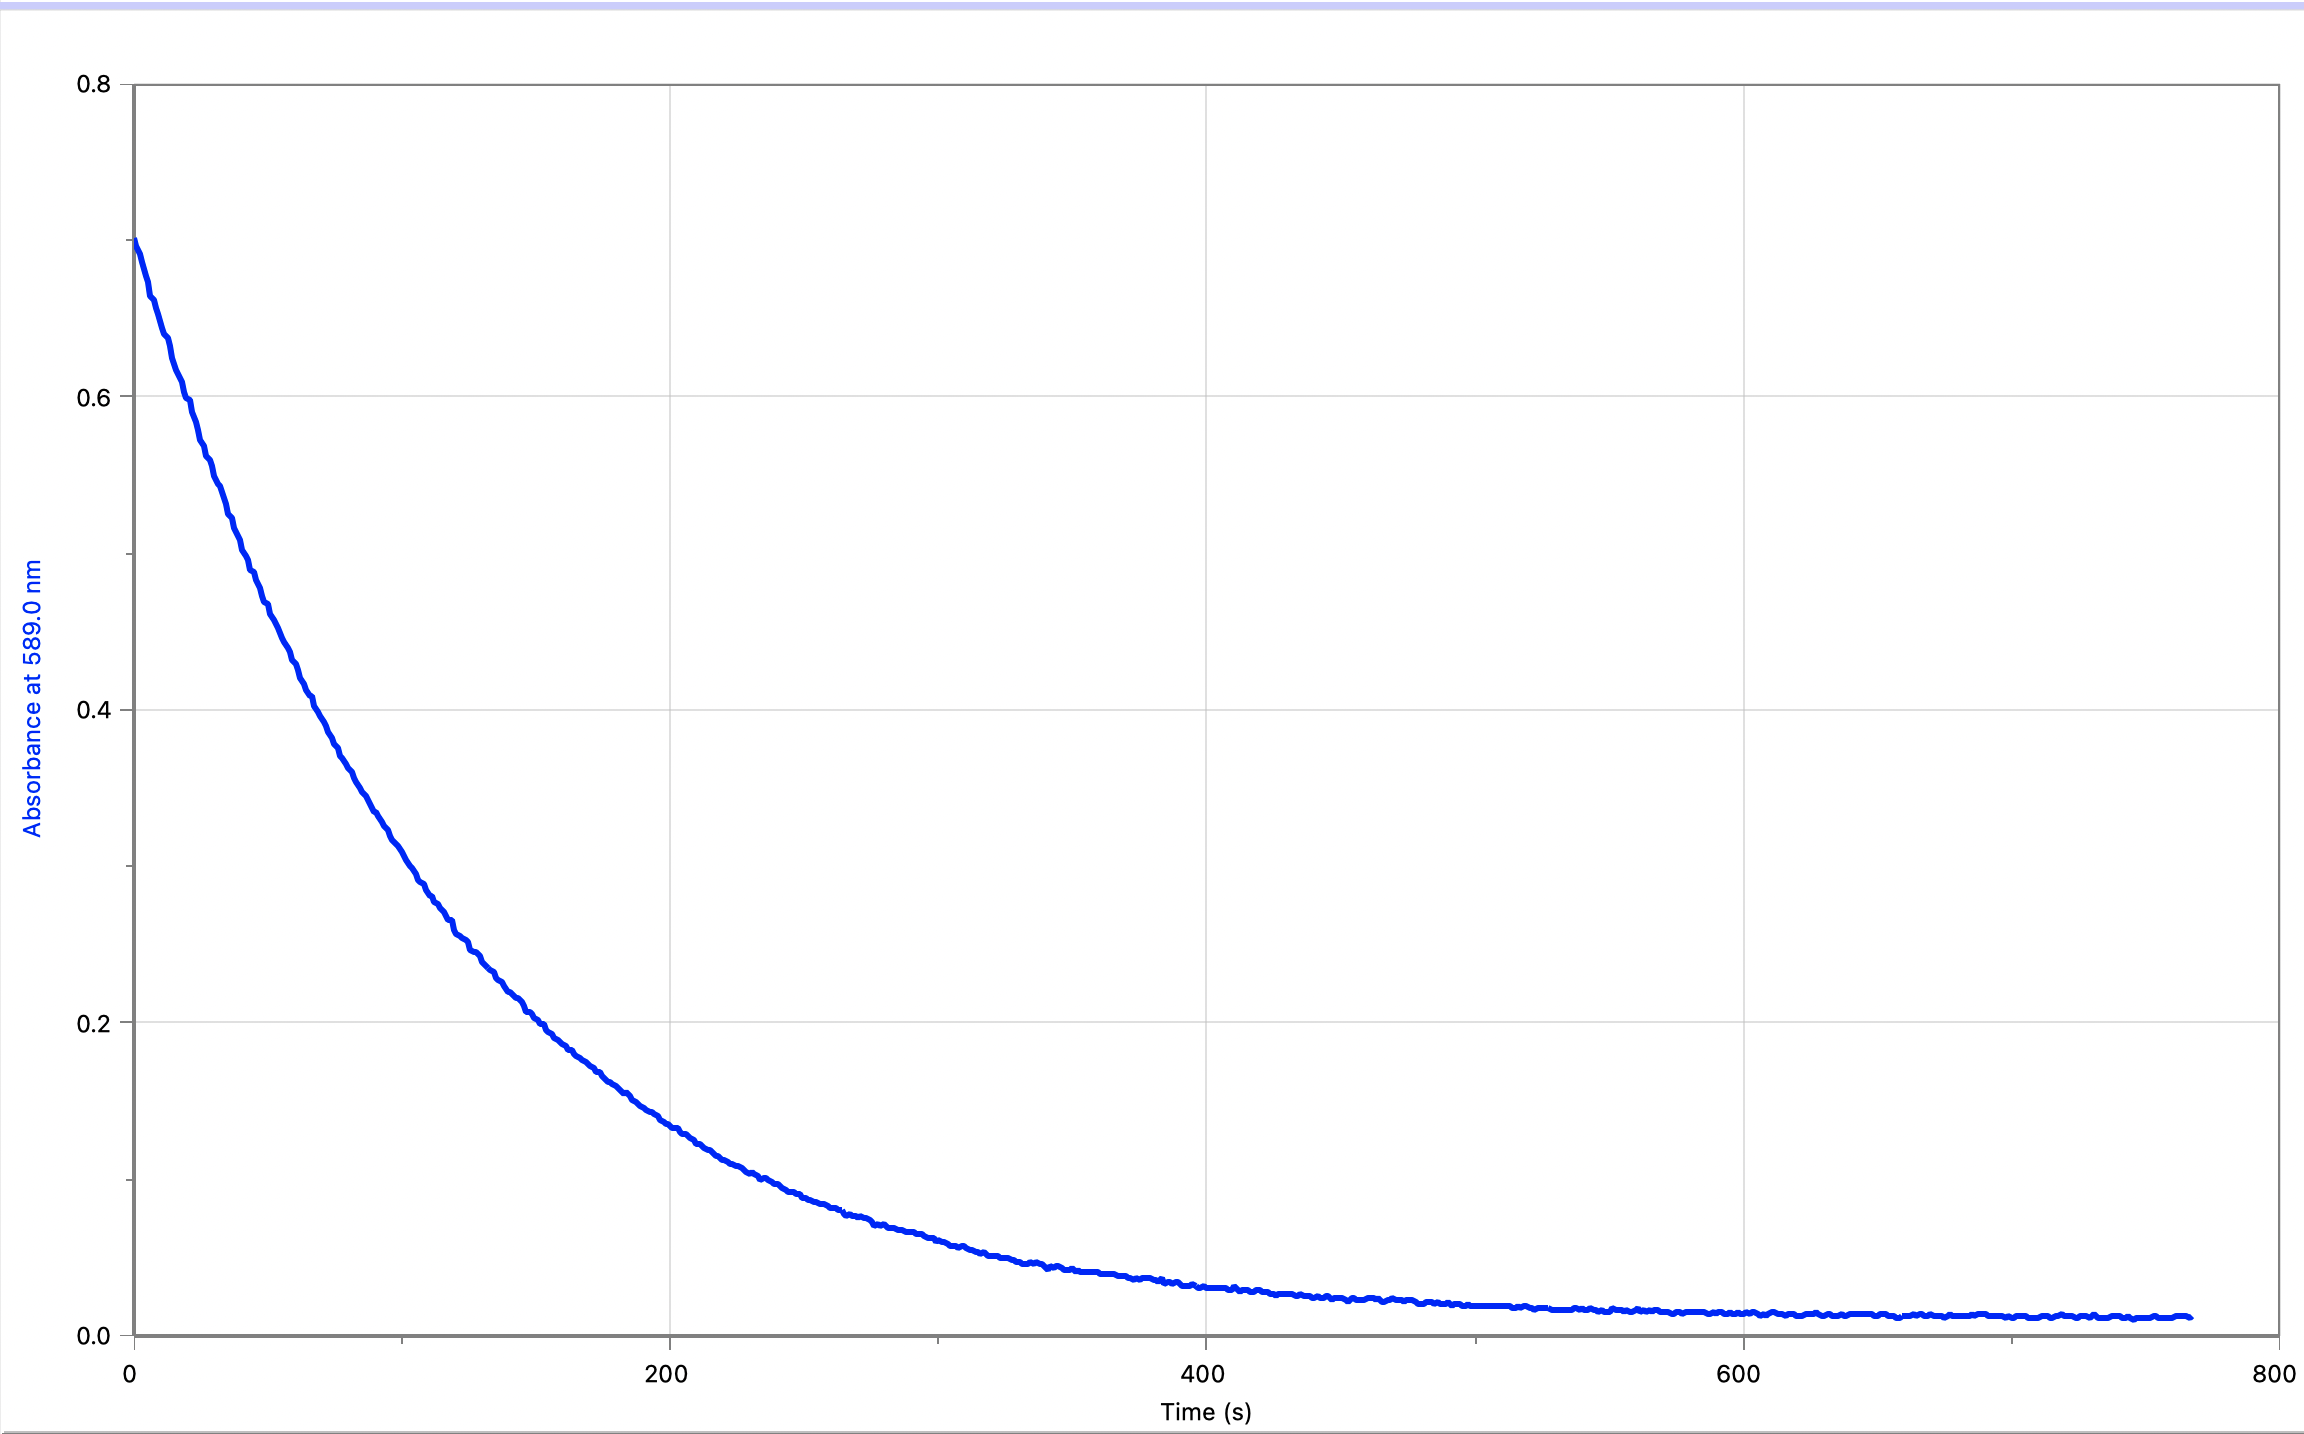
\includegraphics[width=0.85\textwidth]{del1.png}
\end{center}
\caption{$(t,A)$-grafen for del 1 tegnet i Logger Pro}
\label{fig:del1}
\end{figure}
\begin{figure}[H]
\begin{center}
  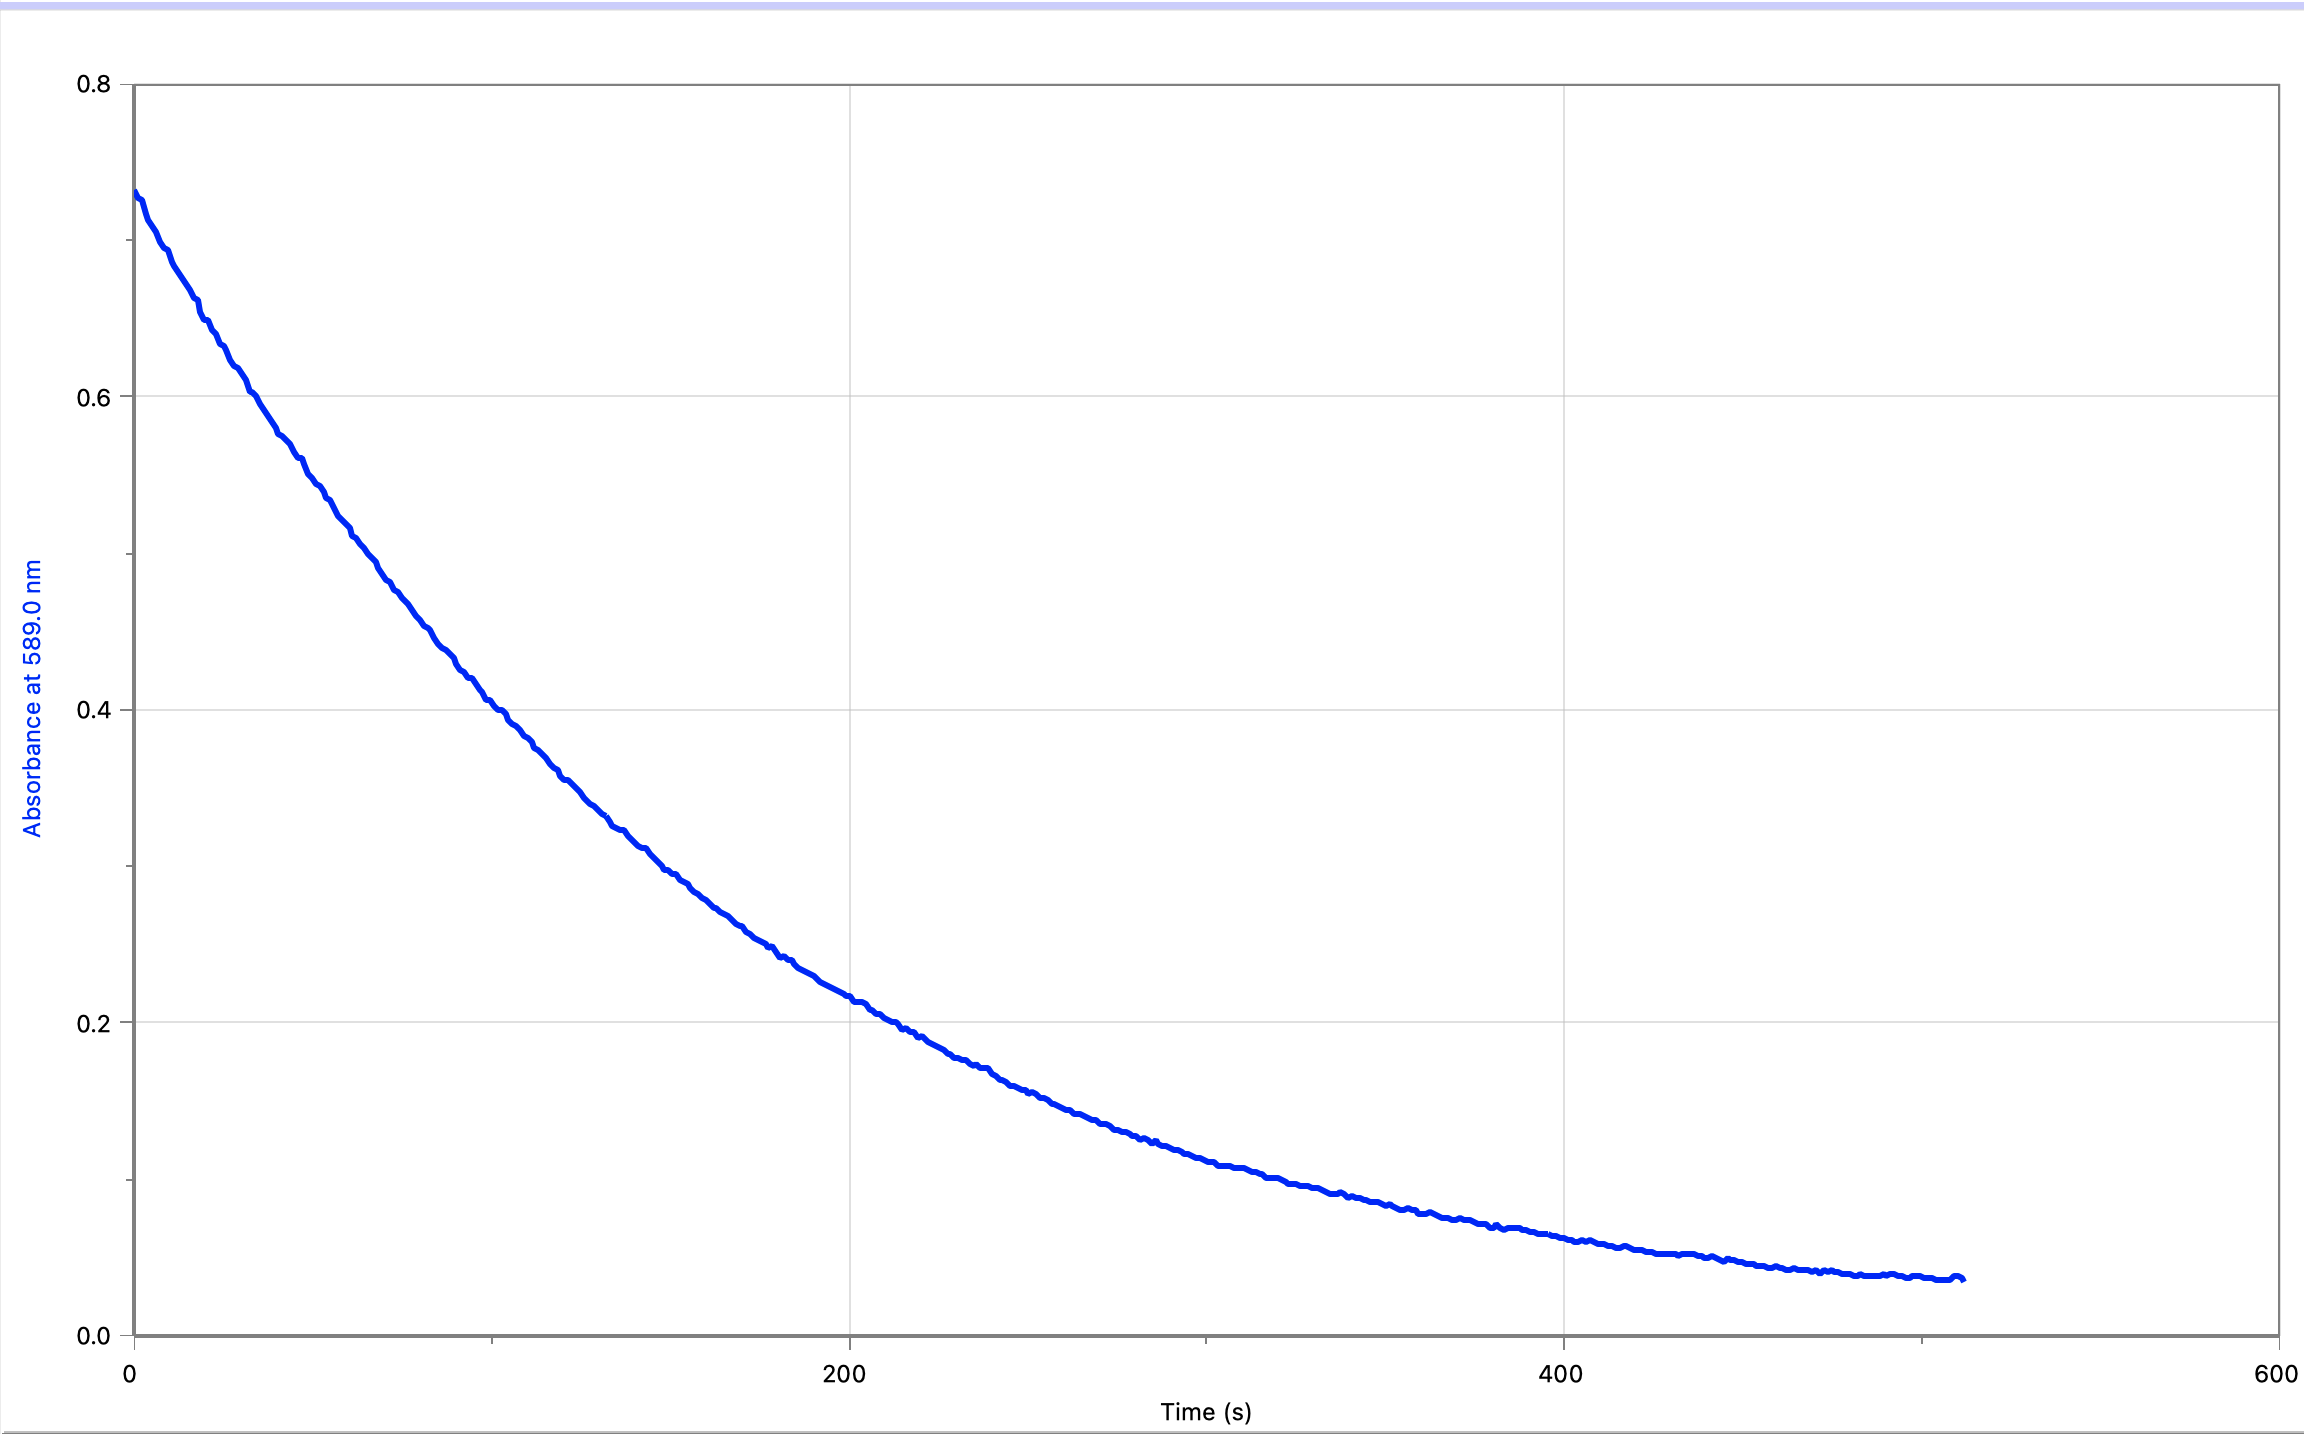
\includegraphics[width=0.85\textwidth]{del2.png}
\end{center}
\caption{$(t,A)$-grafen for del 2 tegnet i Logger Pro}
\label{fig:del2}
\end{figure}

\section*{Efterbehandling og sammenfatning}
Vi vil først bestemme reaktionsordenen mht. krystalviolet.
Vi starter med at betragte $(t,A)$-grafen for del 1.
Hvis reaktionen er af nulte orden mht. krystalviolet, skal målepunkterne tilnærmelsesvist ligge langs en ret linje med negativ hældningskoefficient.
En lineær regression laves derfor, hvilket ses i \cref{fig:tA}.
Betragter man afbildningen, ses det, at punkterne ikke følger den lineære sammenhæng, idet målingerne ved start og slut ligger over tendenslinjen, hvor de midterste målinger ligger under tendenslinjen.
Reaktionen er altså ikke af nulte orden mht. krystalviolet.
\begin{figure}[H]
\begin{center}
  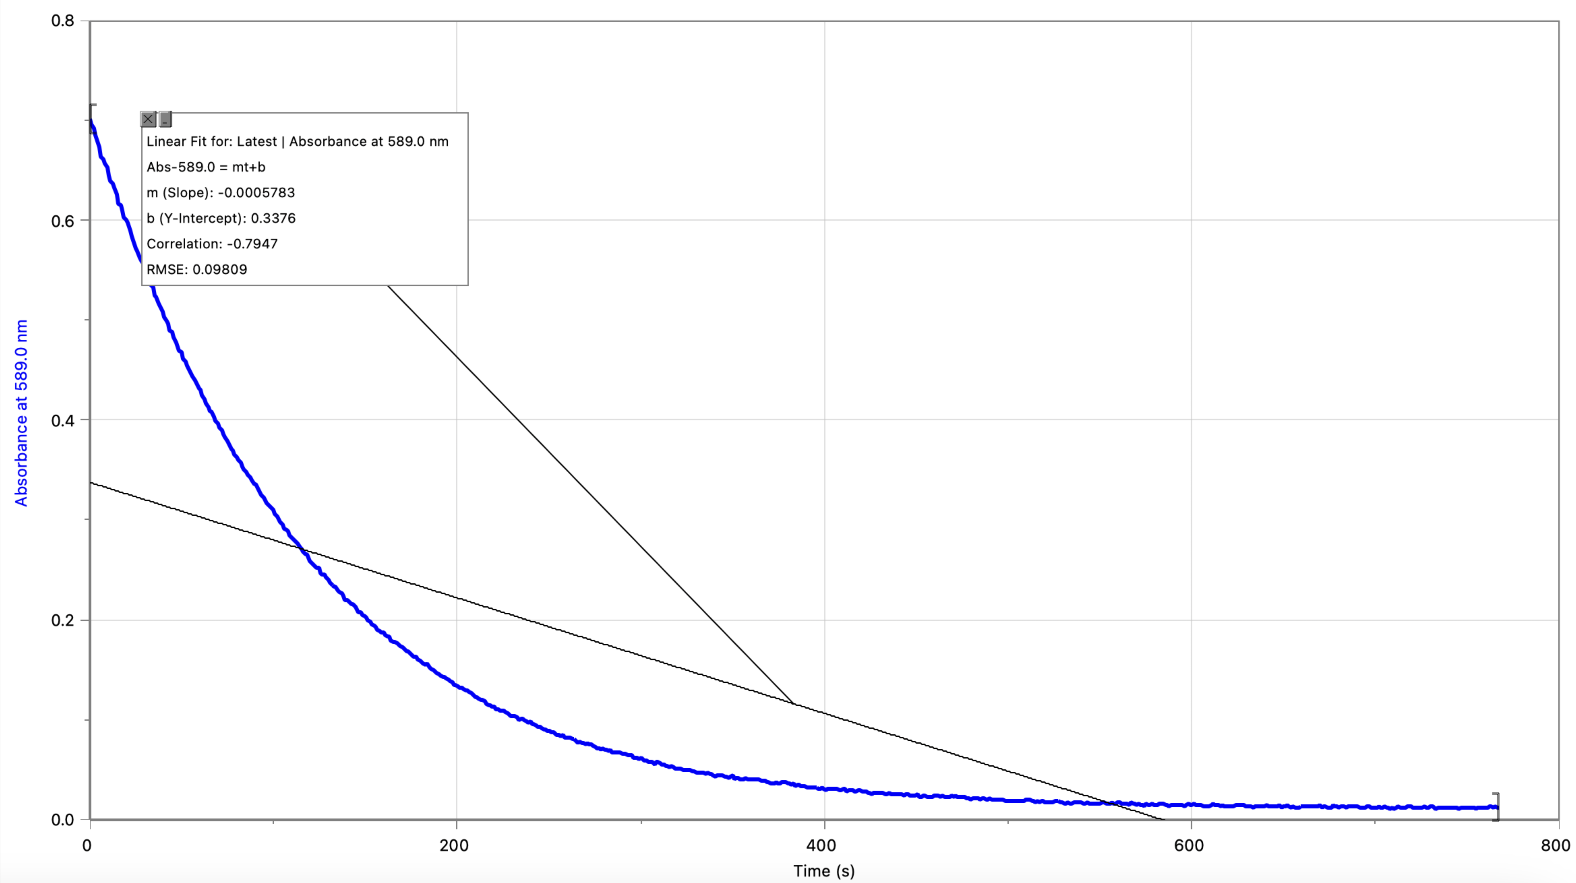
\includegraphics[width=\textwidth]{tA.png}
\end{center}
  \caption{Linær regression med punkterne på $(t,A)$-grafen for del 1}
\label{fig:tA}
\end{figure}
Vi vil nu undersøge, om reaktionen er af første orden mht. krystalviolet.
Hvis reaktionen er af første orden mht. krystalviolet, så gælder der 
\begin{equation}
\begin{split}
  \ln\left[\text{krystalviolet} \right]=-k_1 \cdot t + \ln\left[\text{krystalviolet} \right]_0 &\iff \ln \left( \frac{A}{c}\right)=-k_1 \cdot t + \ln\left(\frac{A_0}{c}\right) \\
  &\iff \ln\left(A\right) - \ln\left(c\right) =-k_1 \cdot t + \ln\left(A_0\right) - \ln\left(c\right) \\
  &\iff \ln\left(A\right) =-k_1 \cdot t + \ln\left(A_0\right) 
\end{split}
  \label{eq:lnA}
\end{equation}
hvor $c=\varepsilon _{\lambda } \cdot l$.
Vi har altså vist, at hvis reaktionen er af første orden mht. krystalviolet, så vil punkterne i $(t,\ln\left(A\right) )$-grafen ligge tilnærmelsesvist på en ret linje.
Vi udfører derfor en lineær regression på $(t,\ln\left(A\right) )$-grafen for del 1, hvilket ses i \cref{fig:tlnA1}.
Målepunkterne sidst i datasættet er ikke medtaget i regressionen, da absorbansen da er så lille, at usikkerheden er meget stor.
\begin{figure}[H]
\begin{center}
  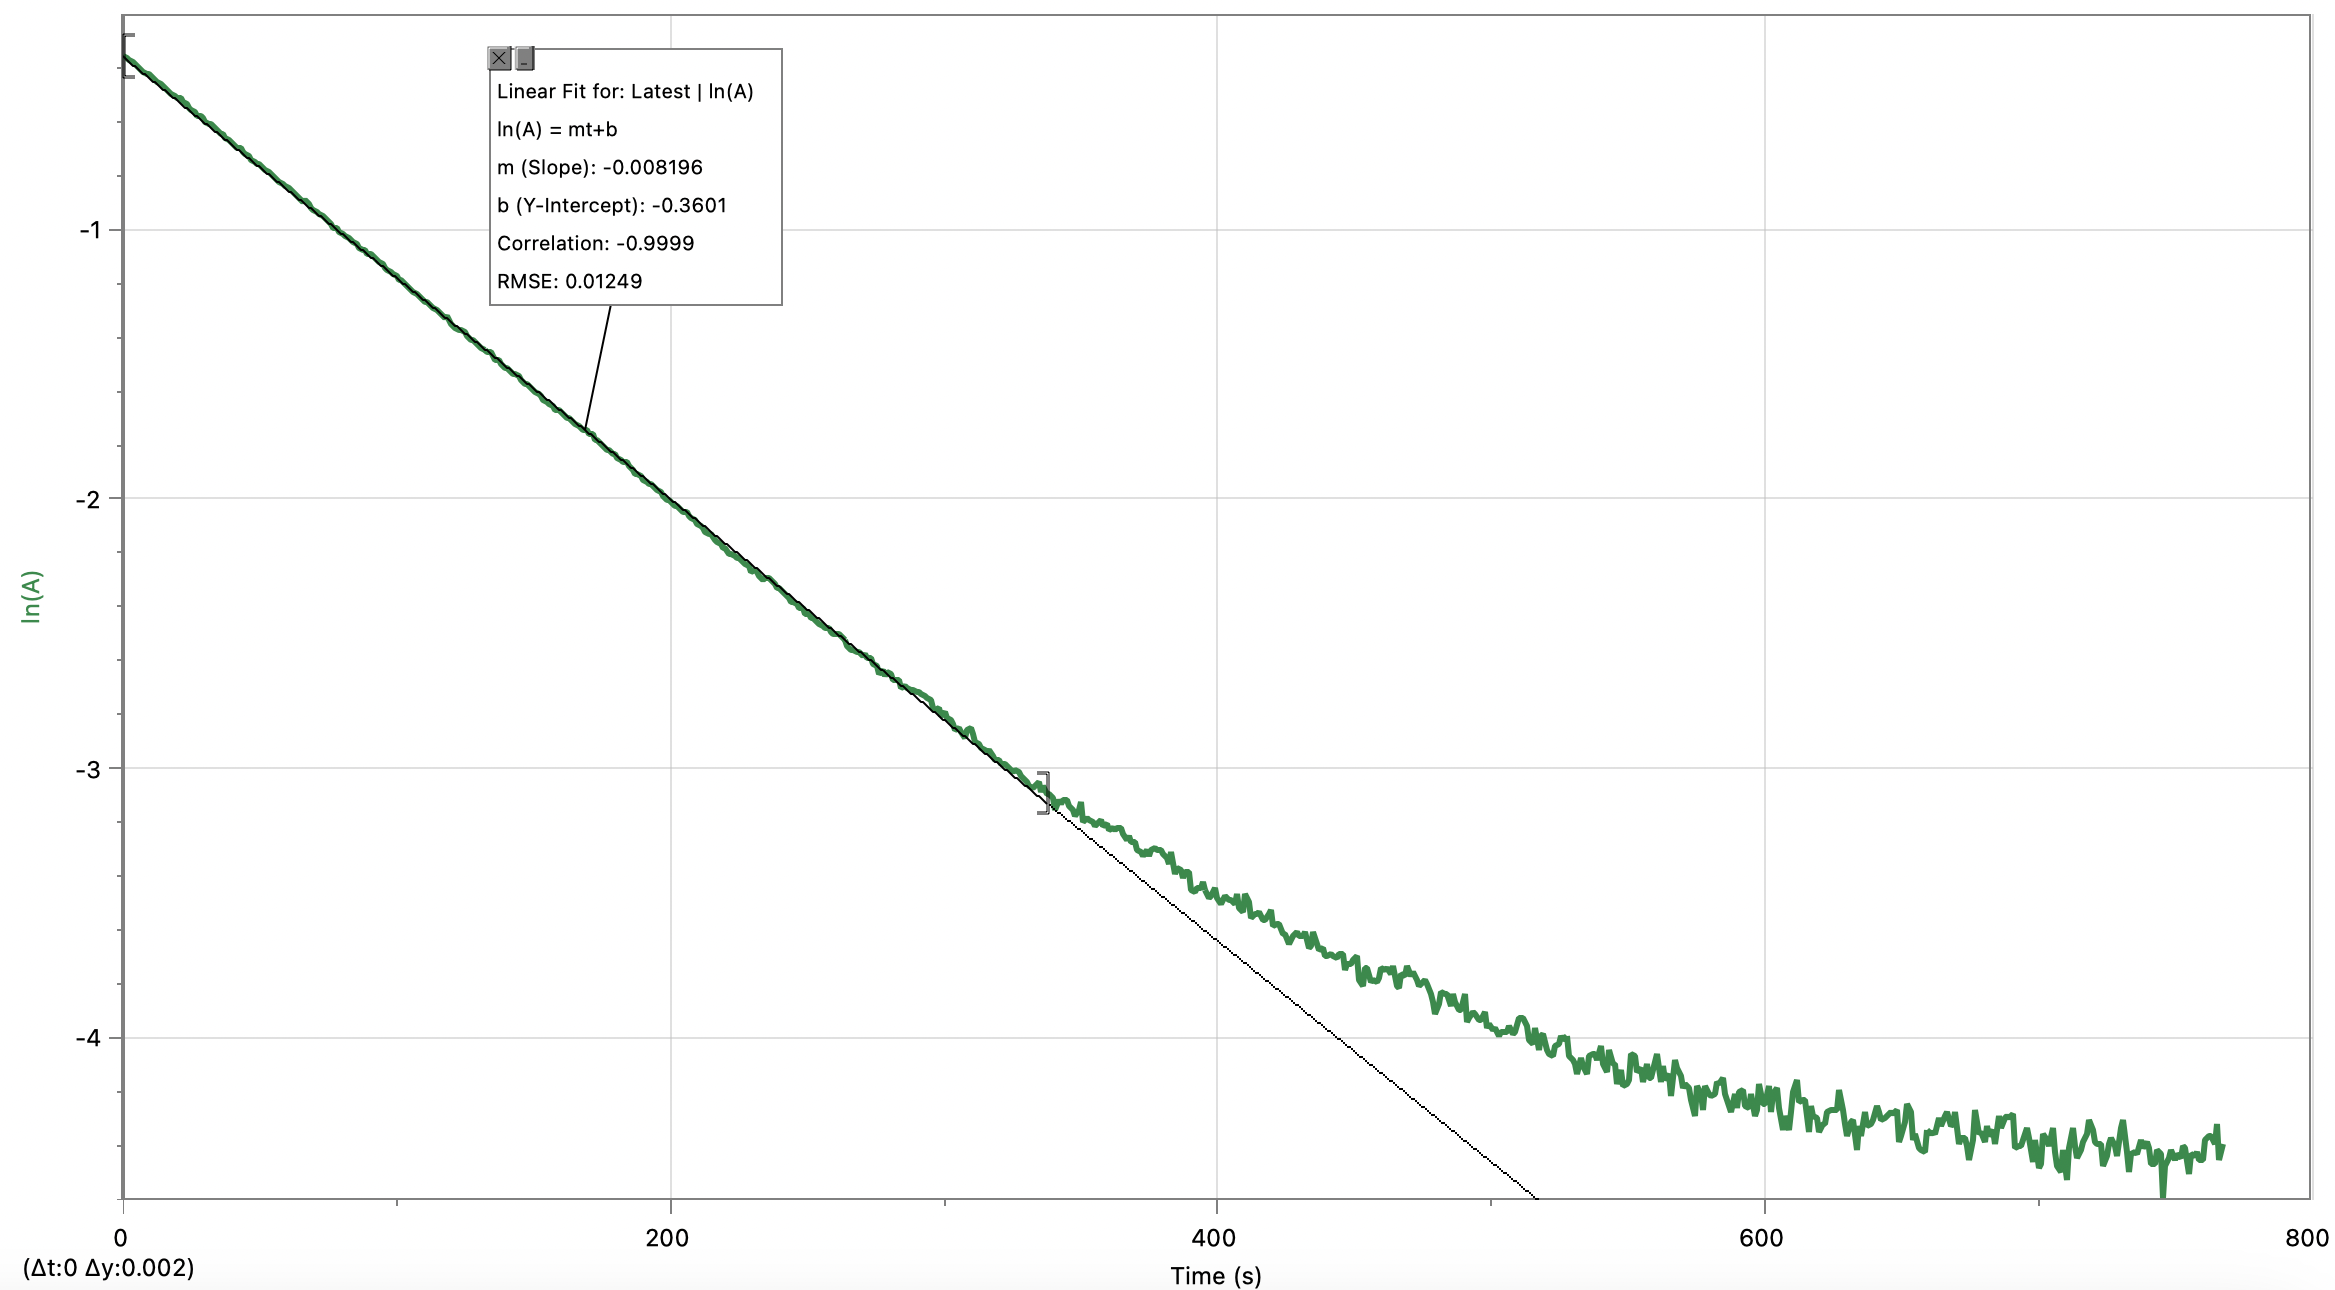
\includegraphics[width=\textwidth]{tlnA1.png}
\end{center}
  \caption{Lineær regression på $(t,\ln\left(A\right)) $-grafen for del 1}
\label{fig:tlnA1}
\end{figure}
Betragter man afbildningen, ses det, at punkterne i starten næsten perfekt følger den lineære sammenhæng.
Det vurderes umiddelbart, at reaktionen er af første orden.
Med andre ord har vi bestemt, at 
\[
x=1
\] 
Fra regressionen har vi derudover, at
\begin{equation}
\ln(A) =-0,008196 \;\unit{s ^{-1}} \cdot t -0,3601
  \label{eq:lnA1}
\end{equation}
For god ordens skyld undersøger vi også, om reaktionen kunne være af anden orden mht. krystalviolet.
Måleresultaterne afbildes da i et $(t,\frac{1}{A})$-diagram, hvor målepunkterne skal ligge tilnærmelsesvist langs en ret linje med positiv hældningskoefficient, hvis reaktionen altså er af anden orden mht. krystalviolet.
En lineær regression laves, hvilket ses i \cref{fig:t1/A}.
\begin{figure}[H]
\begin{center}
  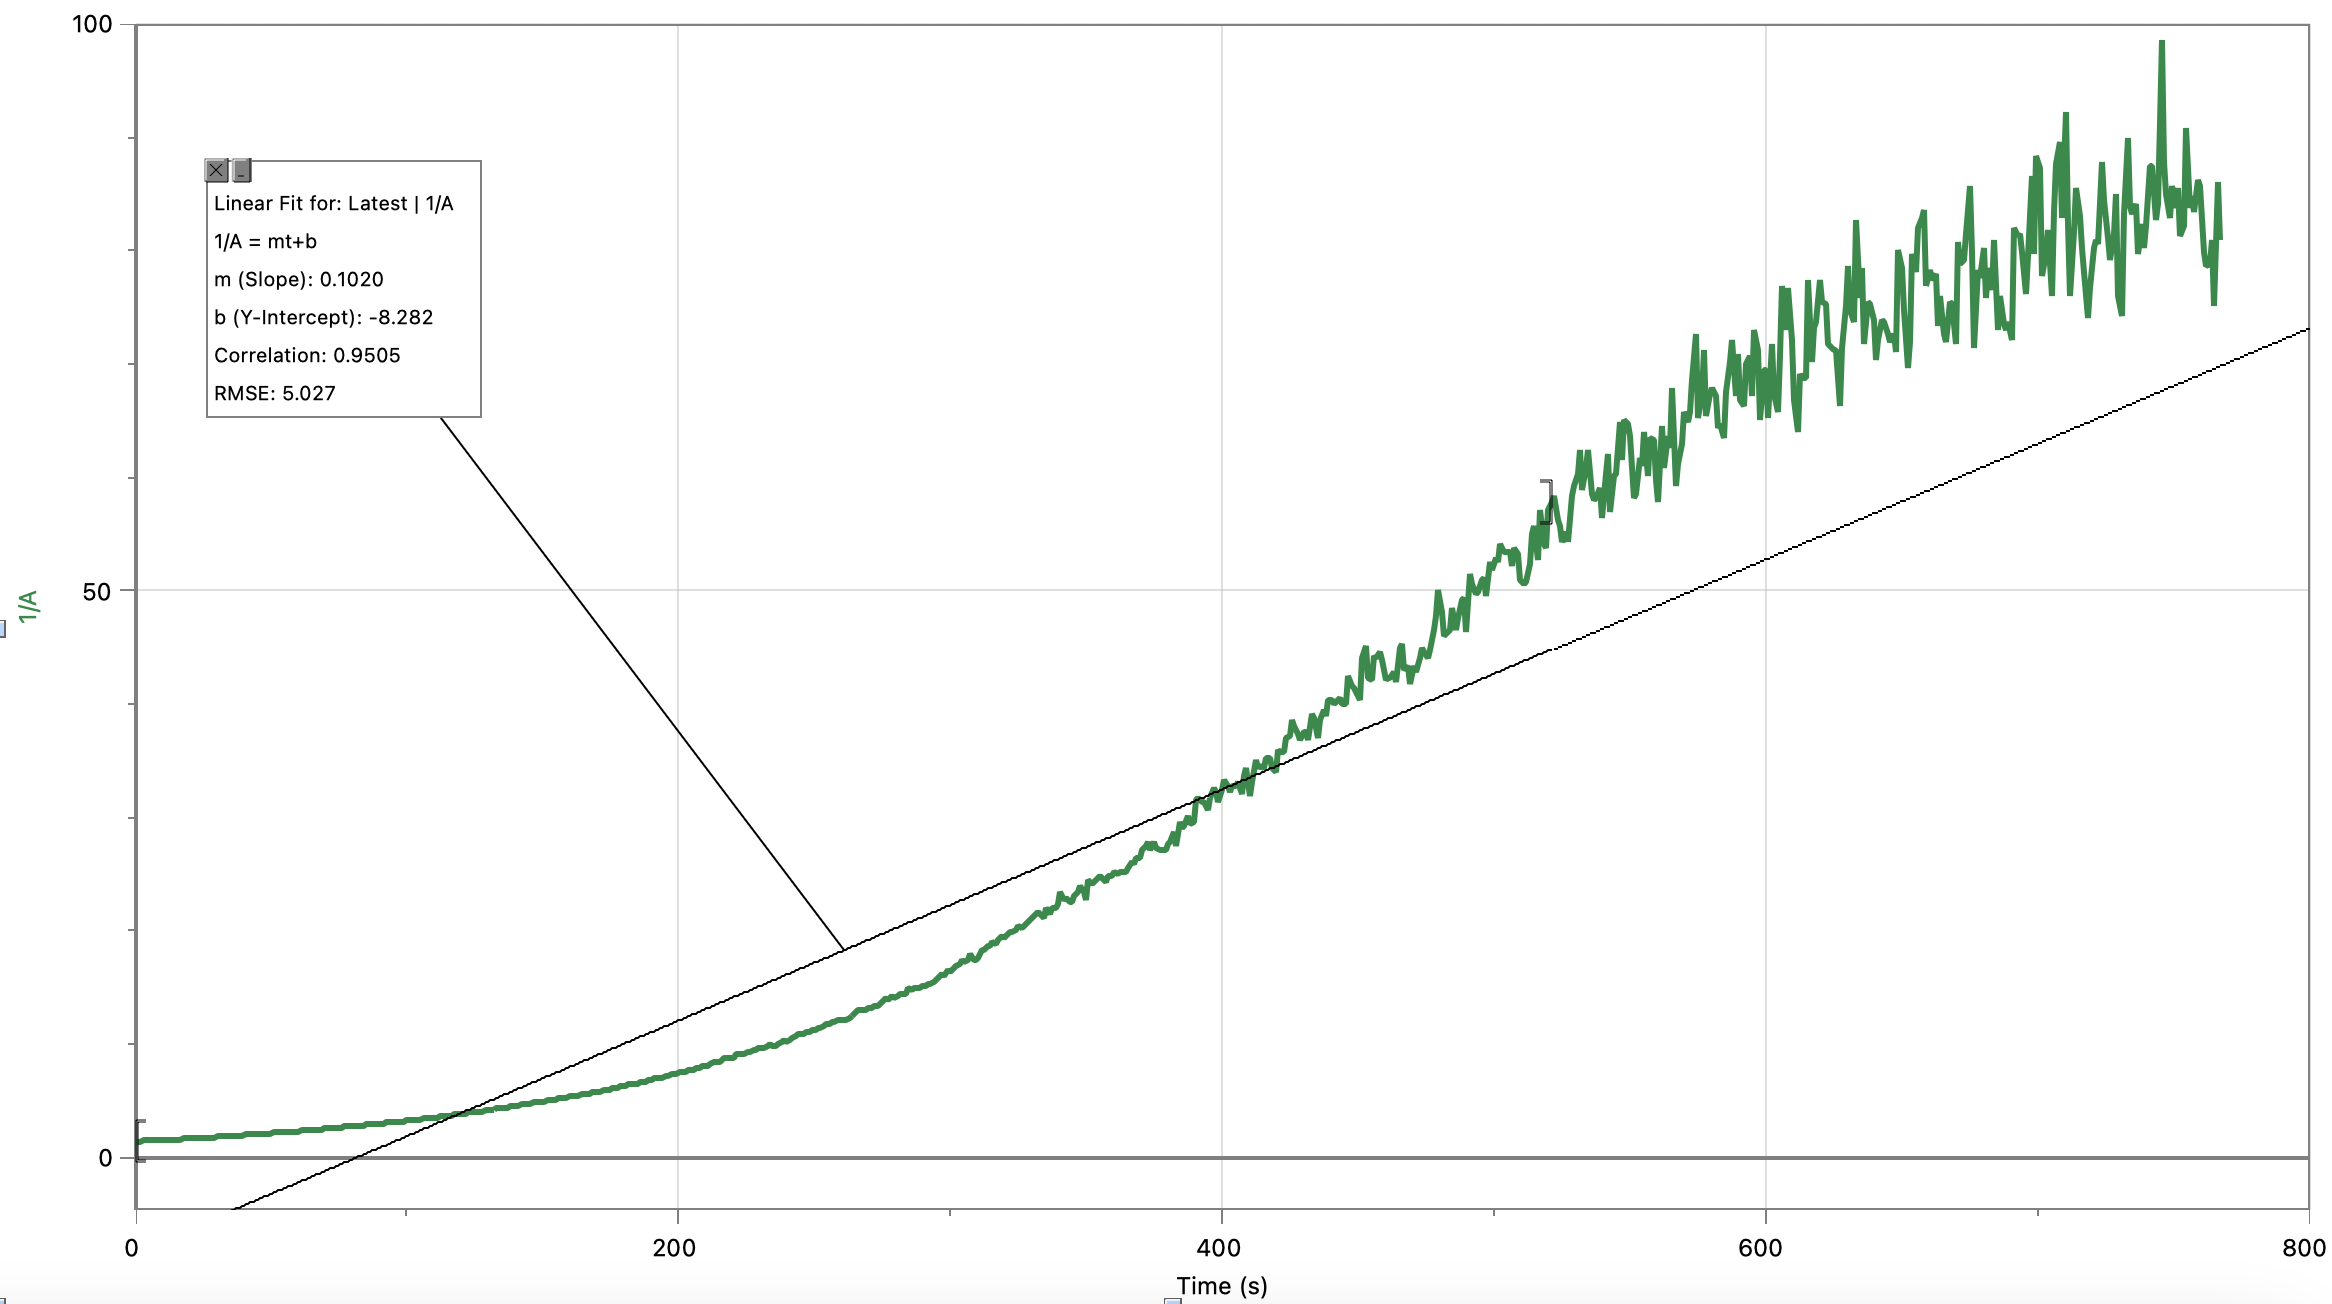
\includegraphics[width=\textwidth]{t1:A.png}
\end{center}
  \caption{Lineær regression på $(t,\frac{1}{A})$-grafen for del 1}
\label{fig:t1/A}
\end{figure}
Som forventet ligger punkterne ikke på en ret linje, heller ikke når vi ser bort fra de sidste målepunkter.
Vi kan altså konkludere, at der er tale om en førsteordensreaktion mht. krystalviolet.

Vi betragter nu $(t, \ln(A))$-grafen for del 2, hvor punkterne også må ligge tilnærmelsesvist på en ret linje, da der jo er tale om en førsteordensreaktion ift. krystalviolet.
Vi laver da en lineær regression, hvilket ses i \cref{fig:tlnA2}.
\begin{figure}[H]
\begin{center}
  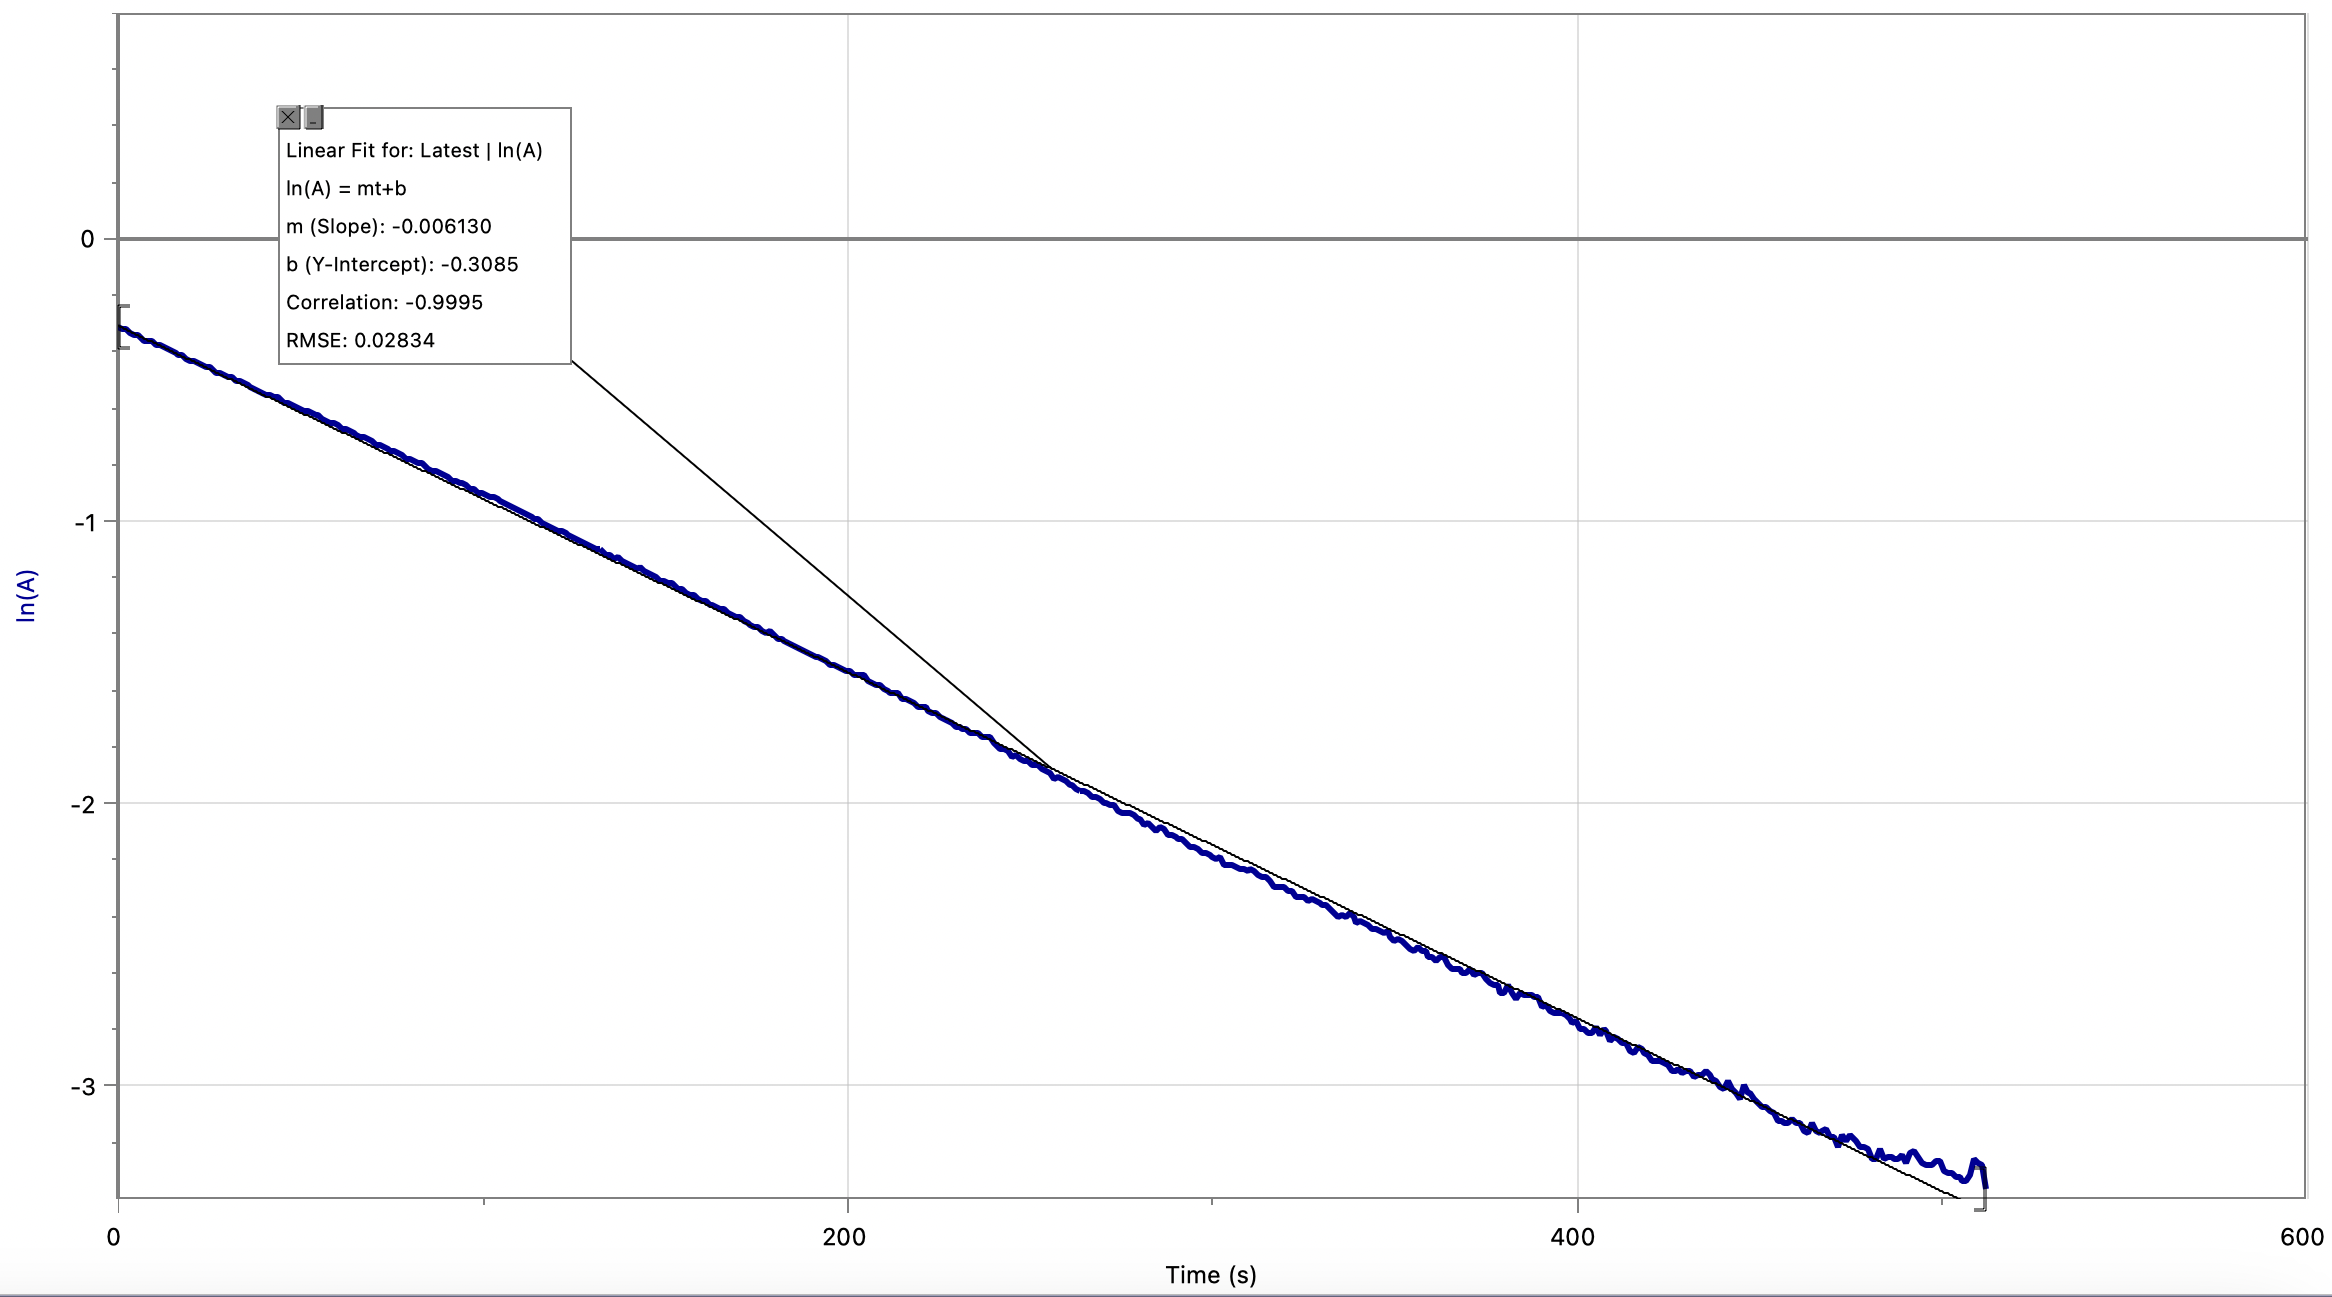
\includegraphics[width=0.9\textwidth]{tlnA2.png}
\end{center}
\caption{Lineær regression på $(t,\ln\left(A\right)) $-grafen for del 2}
\label{fig:tlnA2}
\end{figure}
Det ses, at punkterne ligger tilnærmelsesvist på en ret linje.
Fra den lineære regression har vi, at 
\[
\ln(A)=-0,006130 \;\unit{s ^{-1}} \cdot t -0,3085
\] 
Kombinerer vi dette med ligning \ref{eq:lnA}, er det da nemt at se, at
\[
k_1(\text{del 2} )=0,006130 \;\unit{s ^{-1}} 
\] 
Hvis vi ligeledes kombinerer ligning \ref{eq:lnA} og \ref{eq:lnA1}, får vi 
\[
k_1(\text{del 1} )=0,008196 \;\unit{s ^{-1}} 
\] 
Vi vil nu bestemme reaktionsordenen mht. hydroxid.
Dette gøres ved at finde forholdet mellem $k_1(\text{del 1} )$ og $k_1(\text{del 2} )$.
Teoretisk set har vi nemlig, at 
\begin{equation*}
\begin{split}
  \frac{k_1(\text{del 2} )}{k_1(\text{del 1} )}&=\frac{k \cdot \left(\frac{1}{2} \cdot \left[\ce{OH-} \right]_1\right) ^{y}}{k \cdot \left[\ce{OH-} \right]_1^{y}}\\
  &=\left(\frac{1}{2}\right) ^{y}
\end{split}
\end{equation*}
hvor $\left[\ce{OH-} \right]_1$ er den aktuelle stofmængdekoncentration af hydroxid i del 1. 
Vi beregner da denne størrelse ($y$ beregnes med $\log$ base $\frac{1}{2}$).
\begin{equation*}
\begin{split}
  \frac{k_1(\text{del 2} )}{k_1(\text{del 1} )}&=\frac{0,006130 \;\unit{s ^{-1}} }{0,008196 \;\unit{s ^{-1}} }\\
  &=0,747925817\\
  &\approx \left(\frac{1}{2}\right) ^{0,413}
\end{split}
\end{equation*}
Dette giver imidlertid \textbf{ingen mening}, da $y$ burde være et \textbf{helt tal}.
Den store afvigelse kan skyldes en fejl ved udførelsen af eksperimentet.
En opsummerende tabel ses i \cref{tab:opsum}.
\begin{table}[H]
  \centering
  \begin{tabular}{@{}llll@{}}
  \toprule
  $x$ & $y$ & $k_1(\text{del 1} )$ & $k_1(\text{del 2} )$ \\
  \midrule 
  1 & 0,413 & $0,00820 \;\unit{s ^{-1}} $ & $0,00613 \;\unit{s ^{-1}} $\\ 
  \bottomrule
  \end{tabular}
  \caption{Opsummering vigtigste resultater}
  \label{tab:opsum}
\end{table}
Det (forkerte) generelle hastighedsudtryk for reaktionen ville da være
\[
v= k \cdot \left[\text{krystalviolet} \right]\cdot \left[\ce{OH-} \right] ^{0,413}
\] 
Til slut beregner vi halveringstiden $T _{\frac{1}{2}}$ for krystalviolet i hhv. del 1 og del 2.
Da reaktionsordenen er 1 mht. krystalviolet, så må halveringstiden for krystalviolet i del 1 være
\begin{equation*}
\begin{split}
  T _{\frac{1}{2}}(\text{del 1} )&=\frac{\ln\left(2\right) }{k_1(\text{del 1} )}\\
  &=\frac{\ln\left(2\right) }{0,008196 \;\unit{s ^{-1}} }\\
  &\approx 84,6 \;\unit{s} 
\end{split}
\end{equation*}
Tilsvarende må halveringstiden for krystalviolet i del 2 være
\begin{equation*}
\begin{split}
T _{\frac{1}{2}}(\text{del 2} )&=\frac{\ln\left(2\right) }{k_1(\text{del 2} )}\\
  &=\frac{\ln\left(2\right) }{0,006130 \;\unit{s ^{-1}} }\\
  &\approx 113 \;\unit{s} 
\end{split}
\end{equation*}
Halveringstiden i del 2 ville være dobbelt så stor, hvis reaktionen var af første orden mht. hydroxid.
Dette er dog ikke tilfældet, da vi ikke har fået $y$ til at være et helt tal. 
\section*{Mulige fejlkilder}
En mulig grund til, at vi ikke har fået $y$ som et helt tal kunne være fejl ved pipette-afmålingerne. 
Derudover bliver usikkerheden relativt stor til sidst i de to forsøg, da absorbansen bliver meget lille.

\section*{Konklusion}
Vi har bestemt, at reaktionen er af første orden mht. krystalviolet, men kunne ikke bestemme reaktionsordenen mht. hydroxid, da denne burde være et helt tal.
Skulle vi alligevel opskrive et hastighedsudtryk for krystalviolets reaktion med hydroxid ville det være 
\[
v= k \cdot \left[\text{krystalviolet} \right]\cdot \left[\ce{OH-} \right] ^{0,413}
\] 


\end{document}
